\section{Specification for synchronous experiments}
\label{sec:exp_spec}
In Section~\ref{subsec:sync_exp}, we demonstrate the synchronous experiments with extensive discussions. 
For the reproducibility, we provide here the specification of learning rate grids. The number of iterations as well as epochs, i.e. the number of passes over the full training sets, are also listed for completeness. For \tuner in all the experiments in Section~\ref{sec:experiments}, we uniformly use sliding window size $20$ for extremal curvature estimation and $\beta = 0.999$ for smoothing. For momentum SGD and Adam, we use the following configurations.
\begin{itemize}
	\item CIFAR10 ResNet
		\begin{itemize}
			\item $40$k iterations (${\sim} 114$ epochs)
			\item Momentum SGD learning rates $\{0.001, 0.01 \text{(best)}, 0.1, 1.0\}$, momentum 0.9
			\item Adam learning rates $\{0.0001, 0.001 \text{(best)}, 0.01, 0.1\}$
		\end{itemize}
	\item CIFAR100 ResNet
		\begin{itemize}
			\item $120$k iterations (${\sim} 341$ epochs)
			\item Momentum SGD learning rates $\{0.001, 0.01 \text{(best)}, 0.1, 1.0\}$, momentum 0.9
			\item Adam learning rates $\{0.00001, 0.0001\text{(best)}, 0.001, 0.01\}$
		\end{itemize}
%	\item CIFAR100 ResNext
%		\begin{itemize}
%			\item ${\sim}53$k iterations (${\sim} 40$ epochs)
%			\item Momentum SGD learning rates $\{0.001, 0.01 \text{(best)}, 0.1, 1.0\}$, momentum 0.9
%			\item Adam learning rates $\{0.00001, 0.0001\text{(best)}, 0.001, 0.01\}$
%		\end{itemize}
	\item PTB LSTM
		\begin{itemize}
			\item 30k iterations (${\sim} 13$ epochs)
			\item Momentum SGD learning rates $\{0.01, 0.1, 1.0 \text{(best)}, 10.0\}$, momentum 0.9
			\item Adam learning rates $\{0.0001, 0.001 \text{(best)}, 0.01, 0.1\}$
		\end{itemize}
	\item TS LSTM
		\begin{itemize}
			\item ${\sim}21$k iterations ($50$ epochs)
			\item Momentum SGD learning rates $\{0.05, 0.1, 0.5, 1.0 \text{(best)}, 5.0\}$, momentum 0.9
			\item Adam learning rates $\{0.0005, 0.001, 0.005 \text{(best)}, 0.01, 0.05\}$
			\item Decrease learning rate by factor 0.97 every epoch for all optimizers, following the design by~\citet{karpathy2015visualizing}.
		\end{itemize}
	\item WSJ LSTM
		\begin{itemize}
			\item ${\sim} 120$k iterations ($50$ epochs)
			\item Momentum SGD learning rates $\{0.05, 0.1, 0.5 \text{(best)}, 1.0, 5.0\}$, momentum 0.9
			\item Adam learning rates $\{0.0001, 0.0005, 0.001 \text{(best)}, 0.005, 0.01\}$
			\item Vanilla SGD learning rates $\{0.05, 0.1, 0.5, 1.0 \text{(best)}, 5.0\}$
			\item Adagrad learning rates $\{0.05, 0.1, 0.5 (\text{best}), 1.0, 5.0\}$
			\item Decrease learning rate by factor 0.9 every epochs after 14 epochs for all optimizers, following the design by~\citet{charniakparsing}.
		\end{itemize}
\end{itemize}

\section{Additional experiment results}
\label{sec:add_exp}
\subsection{Training losses on CIFAR10 and CIFAR100 ResNet}
In Figure~\ref{fig:loss_result_cifar}, we demonstrate the training loss on CIFAR10 ResNet and CIFAR100 ResNet. Specifically, \tuner can match the performance of hand-tuned momentum SGD, and achieves 1.93x and 1.38x speedup comparing to hand-tuned Adam respectively on CIFAR10 and CIFAR100 ResNet.
\begin{figure}
\centering
	\begin{tabular}{c c}
		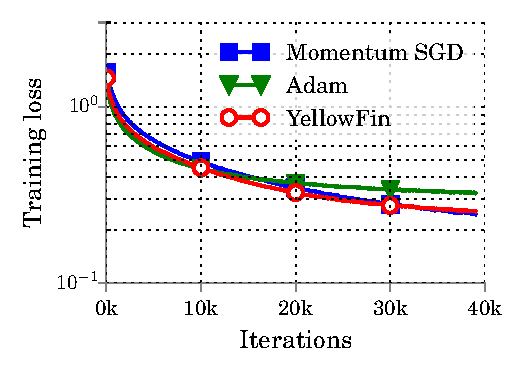
\includegraphics[width=0.4\linewidth]{experiment_results/resnet/resnet_loss.pdf} &
		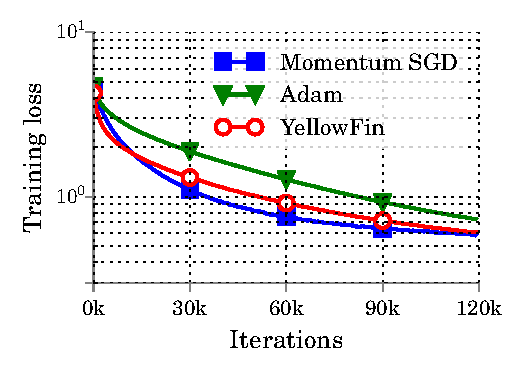
\includegraphics[width=0.4\linewidth]{experiment_results/resnet/resnet_bottleneck_loss.pdf}
	\end{tabular}
	\caption{
	Training loss for ResNet on 100-layer CIFAR10 ResNet (left) and 164-layer CIFAR100 bottleneck ResNet. }
	\label{fig:loss_result_cifar}
\end{figure}

%\subsection{Importance of momentum adaptivity}
%\label{sec:importance_momentum}
%To further emphasize the importance of momentum adaptivity in \tuner, we run YF on CIFAR100 ResNet and TS LSTM. In the experiments, \tuner tunes the learning rate. Instead of also using the momentum tuned by YF, we continuously feed prescribed momentum value $0.0$ and $0.9$ to the underlying momentum SGD optimizer which YF is tuning. In Figure~\ref{fig:cmp_fix_mom}, when comparing to \tuner with prescribed momentum 0.0 or 0.9, \tuner with adaptively tuned momentum achieves observably faster convergence on both TS LSTM and CIFAR100 ResNet. It empirically demonstrates the essential role of momentum adaptivity in \tuner.
%\begin{figure}
%\centering	
%\begin{tabular}{c c}
%	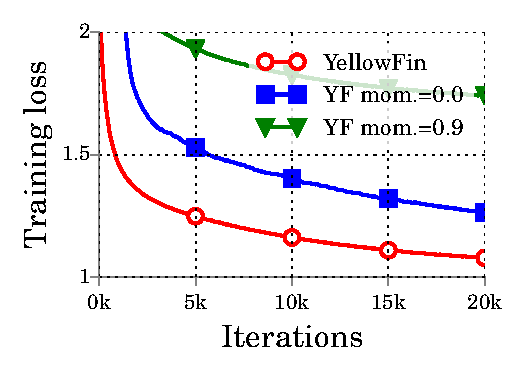
\includegraphics[width=0.4\linewidth]{experiment_results/tf_charrnn_train_loss_fix_mom.pdf} &
%	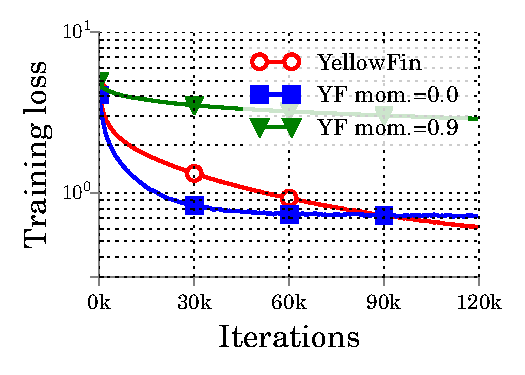
\includegraphics[width=0.4\linewidth]{experiment_results/resnet/resnet_bottleneck_loss_fix_mom_cmp.pdf}
%\end{tabular}
%\caption{Training loss comparison between \tuner with adaptive momentum and \tuner with fixed momentum value. This comparison is conducted on TS LSTM (left) and CIFAR100 ResNet (right).}
%\label{fig:cmp_fix_mom}
%\end{figure}


\subsection{Tuning momentum can improve Adam in asynchronous-parallel setting}
\begin{wrapfigure}[11]{r}{0.31\linewidth}
\vspace{-4.5em}
\begin{minipage}{1.0\linewidth}
	\begin{figure}[H]
		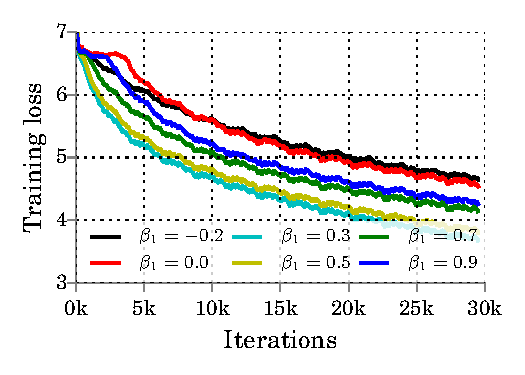
\includegraphics[width=\linewidth]{experiment_results/ptb/adam_stale_15_tuning.pdf}
			\vspace{-1.5em}
		\caption{Hand-tuning Adam's momentum under asynchrony.}
		\label{fig:adam_async_mom}
	\end{figure}
%	\vspace{-1.5em}
%	\begin{figure}[H]
%		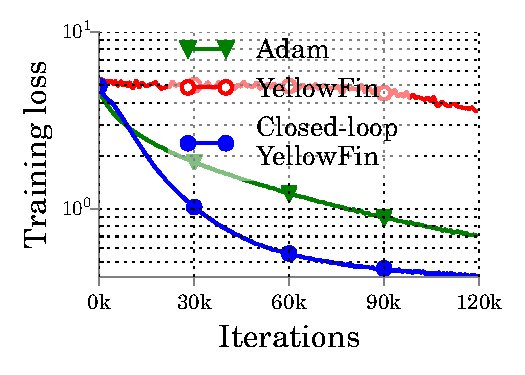
\includegraphics[width=0.975\linewidth]{experiment_results/resnet/resnet_bottleneck_cmp_tuner_adam.pdf}
%%		\caption{Adam, \tuner and \asynctuner on CIFAR100 with 16 async. workers. Sync. baseline uses \tuner.}
%	\vspace{-1.5em}
%		\caption{Asynchronous performance on CIFAR100 ResNet.}
%		\label{fig:full_async_cmp}
%	\end{figure}
\end{minipage}	
\end{wrapfigure}
%\subsection{Asynchronous experiments}
%In this section, we evaulate \tuner in an asynchronous-parallel setting,
%where we focus on {\em statistical efficiency}: the number of iterations to reach a certain solution. 
%To that end, we run $M$ asynchronous workers on a single machine and force them to update the model in a round-robin fashion,
%i.e. the staled gradient is delayed for $(M-1)$ iterations.
%We demonstrate
%%(1) Adam suffers a convergence speed penalty due to not tuning momentum in asynchronous settings;
%(1) \asynctuner (cf.\ Section~\ref{sec:async_tuner}) improves the convergence of \tuner dramatically, which leads to
%(3) \asynctuner having much faster convergence than Adam. 
%\paragraph{State-of-the-art adaptive methods suffer from lack of momentum tuning} 
We conduct experiments on PTB LSTM with 16 asynchronous workers using Adam using the same protocol as in Section~\ref{sec:async_exp}.
Fixing the learning rate to the value achieving the lowest smoothed loss in Section~\ref{subsec:sync_exp}, we sweep the smoothing parameter $\beta_1$~\citep{kingma2014adam} of the first order moment estimate in grid $\{-0.2, 0.0, 0.3, 0.5, 0.7, 0.9\}$. $\beta_1$ serves the same role as momentum in SGD and we call it the momentum in Adam. Figure~\ref{fig:adam_async_mom} shows tuning momentum for Adam under asynchrony gives measurably better training loss. 
This result emphasizes the importance of momentum tuning in asynchronous settings and suggests that state-of-the-art adaptive methods can perform sub-optimally when using prescribed momentum.

\subsection{Accelerating \tuner with finer grain learning rate tuning}
\label{sec:boost_exp}
 As an adaptive tuner, \tuner does not involve manual tuning. It can present faster development iterations on model architectures than grid search on optimizer hyperparameters. In deep learning practice for computer vision and natural language processing, after fixing the model architecture, extensive optimizer tuning (e.g. grid search or random search) can further improve the performance of a model. A natural question to ask is can we also slightly tune \tuner to accelerate convergence and improve the model performance. Specifically, we can manually multiply a positive number, the learning rate factor, to the auto-tuned learning rate in \tuner to further accelerate. 
 
In this section, we empirically demonstrate the effectiveness of learning rate factor on a 29-layer ResNext (2x64d)~\citep{xie2016aggregated} on CIFAR10 and a Tied LSTM model~\citep{press2016using} with 650 dimensions for word embedding and two hidden units layers on the PTB dataset. 
%The architecture of the models are specified in Table~\ref{tab:model_specification} in Appendix~\ref{sec:model_spec}.
 	 When running \tuner, we search for the optimal learning rate factor in grid $\{\frac{1}{3}, 0.5, 1, 2(\text{best for ResNext} ), 3 (\text{best for Tied LSTM} ), 10\}$. 
 	 Similarly, we search the same learning rate factor grid for Adam, multiplying the factor to its default learning rate $0.001$. 
 	 To further strengthen the performance of Adam as a baseline, we also run it on conventional logarithmic learning rate grid $\{5e^{-5}, 1e^{-4}, 5e^{-4}, 1e^{-3}, 5e^{-3}\}$ for ResNext and $\{1e^{-4}, 5e^{-4}, 1e^{-3}, 5e^{-3}, 1e^{-2}\}$ for Tied LSTM. We report the best metric from searching the union of learning rate factor grid and logarithmic learning rate grid as searched Adam results.
 	 Empirically, learning factor $\frac{1}{3}$ and $1.0$ works best for Adam respectively on ResNext and Tied LSTM. 
% 	 To provide another conventional baseline, we also demonstrate the performance from Adam with learning rate search on logarithmic grids. In this grid, we pick the learning rate giving the best validation/test metric. More specifically, we use grid $\{5e^{-5}, 1e^{-4}(\text{best}), 5e^{-4}, 1e^{-3}, 5e^{-3}\}$ for ResNext and $\{1e^{-4}, 5e^{-4}, 1e^{-3} (\text{best}), 5e^{-3}, 1e^{-2}\}$ for Tied LSTM. 
 	 
As shown in Figure~\ref{fig:yf_boost}, with the searched best learning rate factor, \tuner can improve validation perplexity on Tied LSTM from $88.7$ to $80.5$, an improvement of more than $9\%$. Similarly, the searched learning rate factor can improve test accuracy from $92.63$ to $94.75$ on ResNext. More importantly, we can observe, with learning rate factor search on the two models, \tuner can achieve better validation metric than the searched Adam results. It demonstrates that finer-grain learning rate tuning, i.e. the learning rate factor search, can be effectively applied on \tuner to improve the performance of deep learning models.
 	
 	
\begin{figure}
\centering
\begin{tabular}{c c} 
 	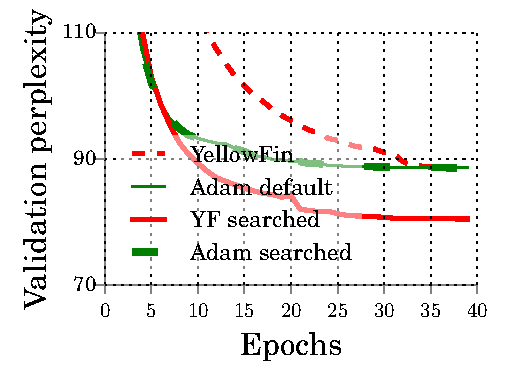
\includegraphics[width=0.4\linewidth]{experiment_results/pytorch_tied_ptb_test_perp_boost_all_seed.pdf} &
 	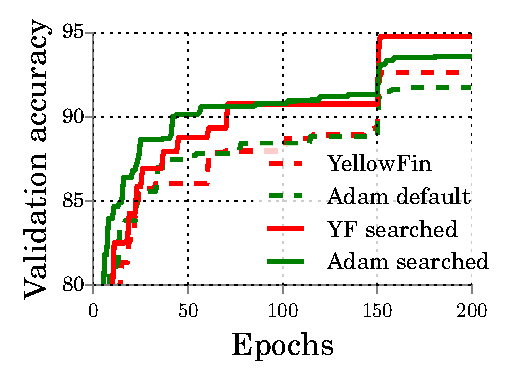
\includegraphics[width=0.4\linewidth]{experiment_results/pytorch_cifar_test_acc_boost.pdf}
\end{tabular}
\caption{Validation perplexity on Tied LSTM and validation accuracy on ResNext. Learning rate fine-tuning using grid-searched factor can further improve the performance of \tuner in Algorithm~\ref{alg:basic-algo}. \tuner with learning factor search can outperform hand-tuned Adam  on validation metrics on both models.}
\label{fig:yf_boost}
\end{figure}





